\let\negmedspace\undefined
\let\negthickspace\undefined
\documentclass[journal]{IEEEtran}
\usepackage[a5paper, margin=10mm, onecolumn]{geometry}
%\usepackage{lmodern} % Ensure lmodern is loaded for pdflatex
\usepackage{tfrupee} % Include tfrupee package

\setlength{\headheight}{1cm} % Set the height of the header box
\setlength{\headsep}{0mm}     % Set the distance between the header box and the top of the text

\usepackage{gvv-book}
\usepackage{gvv}
\usepackage{cite}
\usepackage{amsmath,amssymb,amsfonts,amsthm}
\usepackage{algorithmic}
\usepackage{graphicx}
\usepackage{textcomp}
\usepackage{xcolor}
\usepackage{txfonts}
\usepackage{listings}
\usepackage{enumitem}
\usepackage{mathtools}
\usepackage{gensymb}
\usepackage{comment}
\usepackage[breaklinks=true]{hyperref}
\usepackage{tkz-euclide} 
\usepackage{listings}
% \usepackage{gvv}                                        
\def\inputGnumericTable{}                                 
\usepackage[latin1]{inputenc}                                
\usepackage{color}                                            
\usepackage{array}                                            
\usepackage{longtable}                                       
\usepackage{calc}                                             
\usepackage{multirow}                                         
\usepackage{hhline}                                           
\usepackage{ifthen}                                           
\usepackage{lscape}
\begin{document}

\bibliographystyle{IEEEtran}
\vspace{3cm}

\title{NCERT - 9.4.11}
\author{EE24BTECH11040 - Mandara Hosur}
% \maketitle
% \newpage
% \bigskip
{\let\newpage\relax\maketitle}

\renewcommand{\thefigure}{\theenumi}
\renewcommand{\thetable}{\theenumi}
\setlength{\intextsep}{10pt} % Space between text and floats


\numberwithin{equation}{enumi}
\numberwithin{figure}{enumi}
\renewcommand{\thetable}{\theenumi}

\textbf{Question:}\\
For the differential equation given below, find a particular solution that satisfies y=1 when x=0:
\begin{align}
\brak{x^3 + x^2 + x + 1}\frac{dy}{dx} = 2x^2 + x
\end{align}

\textbf{Solution (using the method of finite differences):} \\
The required particular solution can be found using the method of finite differences. 

\begin{align}
\frac{dy}{dx} = \frac{y(x+h) - y(x)}{h} \\
\implies y(x+h) = y(x) + h\cdot\frac{dy}{dx}
\end{align}

As can be seen from the question above,

\begin{align}
\frac{dy}{dx} = \frac{2x^2 + x}{\brak{x^3 + x^2 + x + 1}} \\
\implies y(x+h) = y(x) + h\cdot\frac{2x^2 + x}{\brak{x^3 + x^2 + x + 1}}
\end{align}

Let $x_0 = 0$ and $y_0 = 1$ (as per the given condition). \\
Let some $x_1 = x_0 + h$. Then
\begin{align}
y_1 = y_0 + h\cdot\frac{2x_0^2 + x_0}{\brak{x_0^3 + x_0^2 + x_0 + 1}}
\label{0.6}
\end{align}

Iterating through the above-mentioned process to generate $y_2$, $y_3$, $y_4$ and so on generalises equation \eqref{0.6} to

\begin{align}
y_{n+1} = y_n + h\cdot\frac{2x_n^2 + x_n}{\brak{x_n^3 + x_n^2 + x_n + 1}}
\end{align}

The smaller the value of $h$, the more accurate the curve is. 

\newpage

\textbf{Solution (using manual methods):}

\begin{align}
\frac{dy}{dx} = \frac{2x^2 + x}{\brak{x^3 + x^2 + x + 1}} \\
\implies \frac{dy}{dx} = \frac{2x^2 + x}{(x^2+1)(x+1)}
\label{0.9}
\end{align}

To split equation \eqref{0.9} into partial fractions, assume that it can be rewritten as given below:
\begin{align}
\frac{dy}{dx} = \frac{A}{x+1} + \frac{Bx + C}{x^2 + 1}
\label{0.10}
\end{align}
Here $A$, $B$, and $C$ are real numbers.

From equation \eqref{0.10},
\begin{align}
\frac{dy}{dx} = \frac{A(x^2+1) + (Bx+C)(x+1)}{(x+1)(x^2+1)} \\
\implies \frac{dy}{dx} = \frac{(A+B)x^2 + (B+C)x + (A+C)}{(x+1)(x^2+1)}
\label{0.12}
\end{align}

Equating equations \eqref{0.9} and \eqref{0.12}, we get
\begin{align}
A = \frac{1}{2} \text{ and } B = \frac{3}{2} \text{ and } C = \frac{-1}{2}
\label{0.13}
\end{align}

Substituting equation \eqref{0.13} in equation \eqref{0.10} and integrating, we get
\begin{align}
\int \,dy = \int \brak{\frac{1}{2(x+1)} + \frac{3x - 1}{2(x^2 + 1)}} \,dx \\
\int \,dy = \frac{1}{2}\int\frac{1}{(x+1)}\,dx + \frac{3}{4}\int\frac{2x}{x^2+1}\,dx - \frac{1}{2}\int\frac{1}{x^2+1}\,dx \\
\implies y = \frac{1}{2}\ln{(x+1)} + \frac{3}{4}\ln{(x^2+1)} - \frac{1}{2}\tan^{-1}{x} + c
\label{0.16}
\end{align}
Here, $c$ is the constant of integration. \\
Substituting the initial conditions of $x=0$ and $y=1$ in equation \eqref{0.16}, we get
\begin{align}
c = 1
\end{align}

Therefore, the equation of the curve found by manual methods is
\begin{align}
y = \frac{1}{4}\ln{\brak{\brak{x+1}^2\brak{x^2+1}^3}} - \frac{1}{2}\tan^{-1}{x} + 1
\end{align}

\newpage

The curve generated using both described methods for the given question, taking $h=0.1$ and running iterations $100$ times is given below.

\begin{figure}[h]
	\centering
	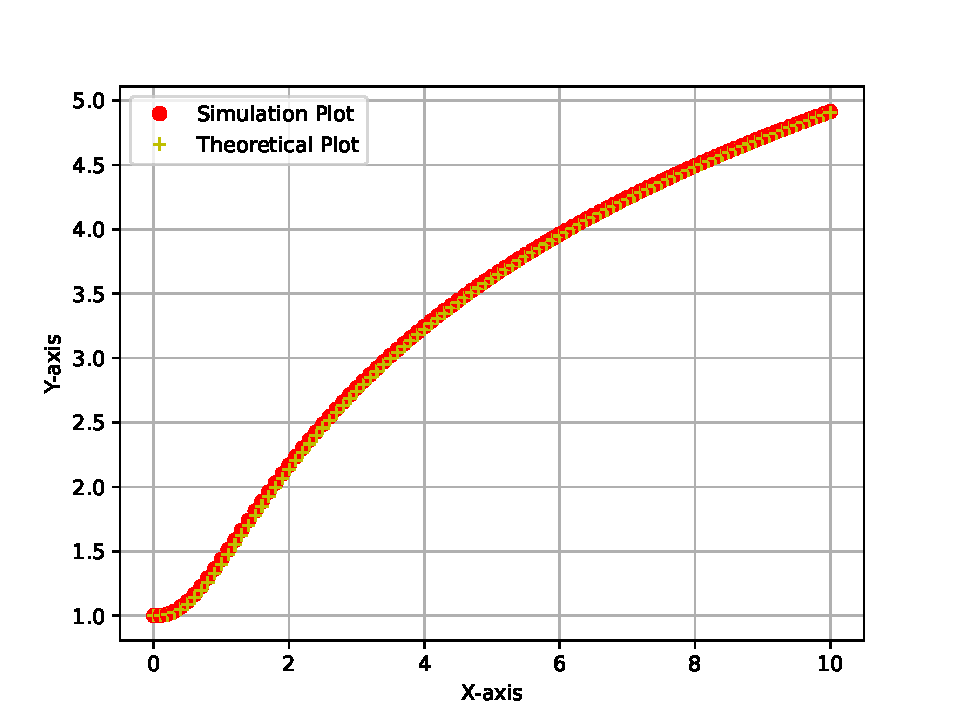
\includegraphics[width=\columnwidth]{figs/fig.pdf}
	\caption{Solution of given DE}
	\label{fig}
\end{figure}

\end{document}
